% Created 2022-01-24 seg 21:27
% Intended LaTeX compiler: pdflatex
\documentclass[letterpaper, 11pt]{article}
                      \usepackage{lmodern} % Ensures we have the right font
\usepackage[T1]{fontenc}
\usepackage[utf8]{inputenc}
\usepackage{graphicx}
\usepackage{amsmath, amsthm, amssymb}
\usepackage[table, xcdraw]{xcolor}
\definecolor{bblue}{HTML}{0645AD}
\usepackage[colorlinks]{hyperref}
\hypersetup{colorlinks, linkcolor=blue, urlcolor=bblue}
\usepackage{titling}
\setlength{\droptitle}{-6em}
\setlength{\parindent}{0pt}
\setlength{\parskip}{1em}
\usepackage[stretch=10]{microtype}
\usepackage{hyphenat}
\usepackage{ragged2e}
\usepackage{subfig} % Subfigures (not needed in Org I think)
\usepackage{hyperref} % Links
\usepackage{listings} % Code highlighting
\usepackage[top=1in, bottom=1.25in, left=1.55in, right=1.55in]{geometry}
\renewcommand{\baselinestretch}{1.15}
\usepackage[explicit]{titlesec}
\pretitle{\begin{center}\fontsize{20pt}{20pt}\selectfont}
\posttitle{\par\end{center}}
\preauthor{\begin{center}\vspace{-6bp}\fontsize{14pt}{14pt}\selectfont}
\postauthor{\par\end{center}\vspace{-25bp}}
\predate{\begin{center}\fontsize{12pt}{12pt}\selectfont}
\postdate{\par\end{center}\vspace{0em}}
\titlespacing\section{0pt}{5pt}{5pt} % left margin, space before section header, space after section header
\titlespacing\subsection{0pt}{5pt}{-2pt} % left margin, space before subsection header, space after subsection header
\titlespacing\subsubsection{0pt}{5pt}{-2pt} % left margin, space before subsection header, space after subsection header
\usepackage{enumitem}
\setlist{itemsep=-2pt} % or \setlist{noitemsep} to leave space around whole list
\author{Vinicius Faria}
\date{\today}
\title{Cálculo 2\\\medskip
\large \emph{Anotações Práticas}}
\hypersetup{
 pdfauthor={Vinicius Faria},
 pdftitle={Cálculo 2},
 pdfkeywords={},
 pdfsubject={},
 pdfcreator={Emacs 27.2 (Org mode 9.5.2)}, 
 pdflang={English}}
\begin{document}

\maketitle
\tableofcontents


\section{Funções Vetoriais}
\label{sec:org587decd}
Funções cuja imagem gerada é um vetor. \(\realbb{R}^2 \ e \ \realbb{R}^3\) são chamadas \textbf{funções coordenadas} e t é denominado \textbf{variável livre}

\begin{center}   $\alpha(t) = (2t+1, 1-t)$ \end{center}

\subsection{Esboço de curvas}
\label{sec:org06b9b73}
Para esboçar curvas, isolar o x e y (e potencialmente z) em função de t, formando a imagem da curva. A curva abaixo descreve um círculo.

\begin{center} $\begin{cases} x(t) = \sin (t) \\ y(t) = \cos(t) \end{cases}$ \end{center}

\subsection{Equações paramétricas de retas}
\label{sec:org991895a}
Dado uma curva que passa por A e B, é possível definir sua função utilizando:

\begin{center} $\alpha (t) = (1-t)A + tB = A + t(B-A)$ \end{center}

Interpretação geométrica: parametrização da reta que contém o ponto A e é parelela ao vetor não nulo (B-A)

\subsection{Parametrizações}
\label{sec:org1bbb194}
Uma função vetorial é uma \uline{parametrização} da curva que é a imagem da função. Uma curva pode ser parametrizada de várias maneiras, como círculos.

\subsection{Limites e Continuidade}
\label{sec:org01c513a}
Resumidamente, para calcular limites de funções vetoriais, basta calcular o limite de cada função de coordenada separadamente.

Da mesma forma, para verificar a continuidade da função vetorial, basta conferir que todas as funções de coordenadas sejam contínuas.

\textbf{OBS:} Uma função é contínua quando em seu domínio:
\begin{itemize}
\item Não possui assíntotas verticais
\item Não possui "furos"
\item Não possui "pulos"
\end{itemize}
\textbf{OBS2:} \(\Vert \alpha (t) \Vert\) denota o módulo do vetor.
\subsection{Derivadas de funções vetoriais}
\label{sec:orge19c020}
A derivada de uma função vetorial é interpretada como o \textbf{vetor tangente ao traço de \(\alpha\) no ponto \(\alpha(a)\)}. Obtida por derivar cada coordenada separadamente

\begin{center} $\alpha(t)' = (\alpha_1'(t), \alpha_2'(t),...)$ \end{center}

Quando a derivada é \(\theta\), gráfico apresenta uma "cúspide". Essa cúspide, no contexto de funções vetoriais, \textbf{não significa que a função é indiferenciável!!!} E sim que o vetor da derivada é equivalente ao vetor nulo.
\begin{center}
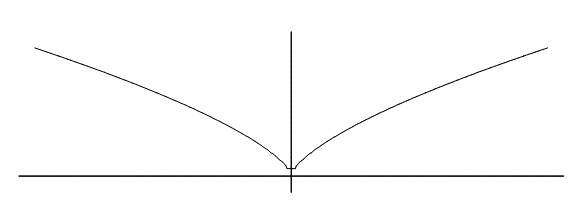
\includegraphics[width=.9\linewidth]{./img/cuspide.png}
\end{center}

\subsubsection{Retas tangentes}
\label{sec:org8bfa222}
Para calcular a reta tangente à função vetorial no ponto a, a derivada é a reta e as coordenadas de \(\alpha\) no ponto a é o ponto inicial.

\begin{center} $r(t) = t\alpha'(a) + \alpha(a)$ \end{center}

No caso de \textbf{coordenadas polares} (tomada por comprimento e angulo de um vetor em vez de coordenadas usuais), utiliza-se:

\begin{center} $\alpha(\theta) = (r(\theta)\cos\theta, r(\theta)\sin\theta)$ \end{center}

\textbf{Exemplo:}

\(\alpha(t) = (t^2, 3t+1) \rightarrow \alpha'(t) = (2t, 3)\)

Então, a reta no ponto \(t = -1\) será

\(t(2\cdot-1, 3) + ((-1)^2,3(-1)+1) \rightarrow (2t+1, 3t+4)\)

No geogebra:
\begin{center}
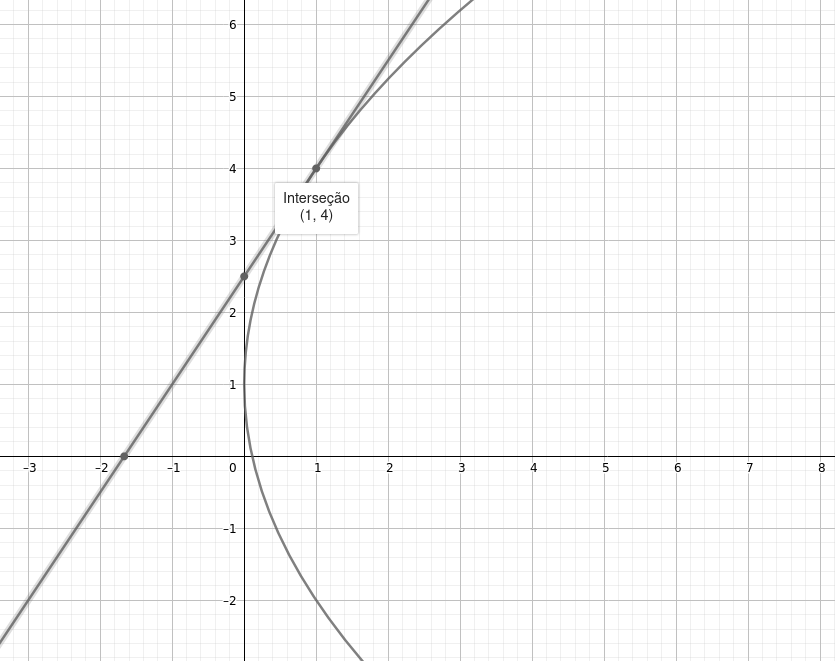
\includegraphics[width=.9\linewidth]{./img/tangente.png}
\end{center}

\textbf{Outro exemplo importante}

Dado a curva \(\alpha(t) = (t^3 +3t, t^2+4t)\), encontrar ponto(s) onde a curva é tangente à reta \(r(t) = (3t+3,t-4)\)

Passo-a-passo: Derivar a curva, encontrar pontos em que essa derivada é paralela ao vetor diretor da reta, isto é: \(\alpha'(t) = \lambda(3,1)\). Solucionar num sistema linear. (Gabarito \(t = -1, t = 3\))

\subsection{Integrais de funções vetoriais}
\label{sec:org7361aeb}
Integrar uma função vetorial é feito da mesma maneira que na derivação: integrando um a um. Realizando a integração indefinida, obtemos a função primitiva de cada uma das coordenadas, sendo útil para descobrir a velocidade através da aceleração, por exemplo.
Por outro lado, a integração definida resulta num vetor. Uma nomenclatura comum no caso da integração até \(\realbb{R}^3\) é separar as coordenadas em \(\vec{i}, \vec{j} \ e \ \vec{k}\) para representar x,y e z.

\begin{center} $\int_{a}^{b} \alpha(t) \ dt = \int_{a}^{b} \alpha_1(t) \ dt \ \vec{\textbf{i}} + \int_{a}^{b} \alpha_2(t) \ dt \ \vec{\textbf{j}} +  \int_{a}^{b} \alpha_3(t) \ dt \ \vec{\textbf{k}}  $ \end{center}

\subsubsection{Comprimento de uma curva}
\label{sec:org28d1479}
Tomando a ideia de módulo de vetores com o somatório da integral, levando em conto que \(\alpha\) é uma função de classe \(C^1\) (Continua e derivável em todos os pontos) tomamos a fórmula:

\begin{center} $L(\alpha) = \int_{a}^{b} |\alpha'(t)| dt \ , \ |\alpha'(t)| = \sqrt{(\alpha_1'(t))^2 + (\alpha_2'(t))^2}$ \end{center}

\subsubsection{Curvas em coordenadas polares}
\label{sec:orgaae76d7}
A fórmula do comprimento de uma curva dada, caso \(r(\theta)\) seja de classe \(C^1\), pela equação \(r = r(\theta)\) é:

\begin{center} $L =\int_{a}^{b} \sqrt{(\dfrac{dr}{d\theta})^2 + r^2 d\theta}$ \end{center}

A fórmula da área da região delimitada por \(0 \le r \le r(\theta), a < \theta < b\) é

\begin{center} $A =\frac{1}{2} \int_{a}^{b} r(\theta)^2 d\theta$ \end{center}

\begin{center}
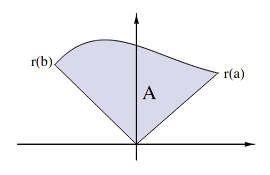
\includegraphics[width=.9\linewidth]{./img/areapolar.png}
\end{center}
\end{document}